%!TEX TS-program = xelatex

% Официальный шаблон презентации НИУ ВШЭ в beamer (LaTeX)
% Версия 2.0
% Язык — русский   
% Автор шаблона - Данил Фёдоровых (fedorovykh@gmail.com)

%%% Для корректной работы шаблона необходима 
%%% установка в систему бесплатного шрифта HSE Sans
%%% https://www.hse.ru/info/brandbook/#font


\documentclass[aspectratio=169]{beamer}

\newbool{russian}
\booltrue{russian}  % Загружает русскоязычный логотип ВШЭ
\usepackage{HSE-theme/beamerthemeHSE} % Подгружаем тему

%%% Работа с русским языком и шрифтами
\usepackage[english,russian]{babel}   % загружает пакет многоязыковой вёрстки
\usepackage[no-math]{fontspec}      % подготавливает загрузку шрифтов Open Type, True Type и др.
	\setsansfont{HSE Sans} 
	\setmonofont{Liberation Mono}
\usepackage{mathspec}
	\setmathsfont(Digits,Latin,Greek)[Numbers={Lining,Proportional}]{HSE Sans}
	\setmathrm[Numbers={Lining,Proportional}]{HSE Sans}
\uselanguage{russian}
\languagepath{russian}
\deftranslation[to=russian]{Theorem}{Теорема}
\deftranslation[to=russian]{Definition}{Определение}
\deftranslation[to=russian]{Definitions}{Определения}
\deftranslation[to=russian]{Corollary}{Следствие}
\deftranslation[to=russian]{Fact}{Факт}
\deftranslation[to=russian]{Example}{Пример}
\deftranslation[to=russian]{Examples}{Примеры}

\usepackage{blindtext} 		% Случайный текст
\usepackage{booktabs} 		% Таблицы
\usepackage{array} 			% Настройка колонок таблиц
\usepackage{colortbl} 		% Цветные строки таблиц
\graphicspath{{images/}}  	% Папка с картинками
\newcommand{\MetricLegend}{%
\vfill
{\fontsize{6.8}{8}\selectfont
	\begin{itemize}
		\setlength{\itemsep}{0.01cm}
		\item \textit{BinaryAcc} --- точность бинарного различения исходных и искажённых графов.
		\item \textit{IntraAcc} --- точность упорядоченных пар \textit{clean/corrupted} в рамках одного трека.
		\item \textit{InterAcc} --- точность упорядоченных пар \textit{clean/corrupted} с разными треками.
	\end{itemize}
}
}

%%% Информация об авторе и выступлении
\title[Заголовок]{Заголовок презентации (если длинный, то в две-три строки)} 
\subtitle{Подзаголовок презентации}
\author[Имя автора]{Имя автора \\ \smallskip \scriptsize author@hse.ru\\\url{http://hse.ru/staff/author/}}
\institute{Название подразделения одну, две или три строки}
\date{\today}

\begin{document}	% Начало презентации

\begin{frame}
\frametitle{GNN Critic}
\framesubtitle{HookTheory Dataset}
\vspace{0.2cm}
	 \begin{columns}[c,totalwidth=\textwidth]
	 \column{0.42\textwidth}
		{\fontsize{15}{19}\selectfont
		\textbf{Всего песен:} 26 178\\[0.25cm]
		\textbf{Количество уникальных}\\
		\textbf{исполнителей:} 6 207\\[0.25cm]
		\textbf{Всего нот:} 1 338 346\\[0.25cm]
		\textbf{Всего аккордов:} 449 072}
		\column{0.58\textwidth}
		\begin{center}
			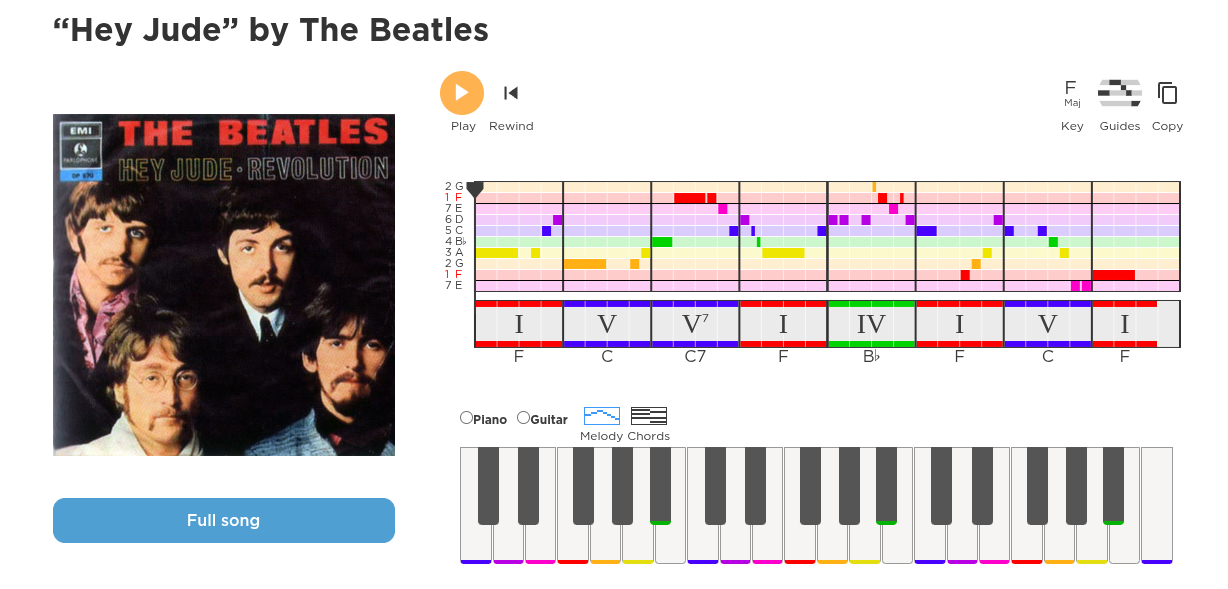
\includegraphics[width=\columnwidth,height=0.56\textheight,keepaspectratio]{image1}\\[0.12cm]
			{\fontsize{14}{17}\selectfont \href{https://www.hooktheory.com/}{HookTheory.com}}
		\end{center}
	\end{columns}
\end{frame}

\begin{frame}
\frametitle{GNN Critic}
\framesubtitle{HookTheory Dataset}
\vspace{0.05cm}
\definecolor{ChordInversion}{RGB}{105,105,105}
\definecolor{ChordAlteration}{RGB}{160,55,55}
\definecolor{ChordOmit}{RGB}{105,65,150}
\definecolor{ChordBorrowed}{RGB}{0,120,120}
\definecolor{ChordApplied}{RGB}{0,115,170}
	 \begin{columns}[T,totalwidth=\textwidth]
	 \column{0.62\textwidth}
		{\fontsize{12.5}{16}\selectfont\raggedright
		\textbf{Каждый клип --- JSON-объект типа:}\\[0.25cm]
		\begin{itemize}
			\setlength{\itemsep}{0.2cm}
			\item \texttt{meta}: \texttt{split}, \texttt{key}, \texttt{tempo}, \texttt{meter}
			\item \texttt{[melody]}: \texttt{beat}, \texttt{duration}, \texttt{scale}, \texttt{degree}, \texttt{octave}, \texttt{rest flag}
			\item \texttt{[chords]}: \texttt{beat}, \texttt{duration}, \textcolor{HSEblue}{\texttt{root}}, \textcolor{HSEgreen}{\texttt{type}}, \textcolor{ChordInversion}{\texttt{inversion}}, \textcolor{ChordApplied}{\texttt{applied}}, \textcolor{HSEorange}{\texttt{adds}}, \textcolor{ChordOmit}{\texttt{omits}}, \textcolor{ChordAlteration}{\texttt{alterations}}, \texttt{suspensions}, \textcolor{ChordBorrowed}{\texttt{borrowed}}, \texttt{rest flag}
		\end{itemize}
		}
		\column{0.38\textwidth}
		\begin{center}
			{\fontsize{28}{34}\selectfont
			\textcolor{HSEblue}{C}%
			\textcolor{HSEgreen}{maj7}%
			\textcolor{HSEorange}{add9}}\\[0.28cm]
			{\fontsize{28}{34}\selectfont
			\textcolor{HSEblue}{A}%
			\textcolor{HSEred}{sus4}}\\[0.28cm]
			{\fontsize{28}{34}\selectfont
			\textcolor{HSEblue}{D}%
			\textcolor{HSEgreen}{7}%
			\textcolor{ChordApplied}{/V}}\\[0.45cm]
			{\fontsize{10}{12}\selectfont
			\textcolor{HSEblue}{root}\quad
			\textcolor{HSEgreen}{type}\quad
			\textcolor{HSEorange}{adds}\quad
			\textcolor{HSEred}{suspensions}\\[0.08cm]
			\textcolor{ChordApplied}{applied}}
		\end{center}
	\end{columns}
\end{frame}

\begin{frame}
\frametitle{GNN Critic}
\framesubtitle{Графовое представление данных}
\vspace{0.05cm}
	 \begin{columns}[c,totalwidth=\textwidth]
	 \column{0.5\textwidth}
		\begin{center}
			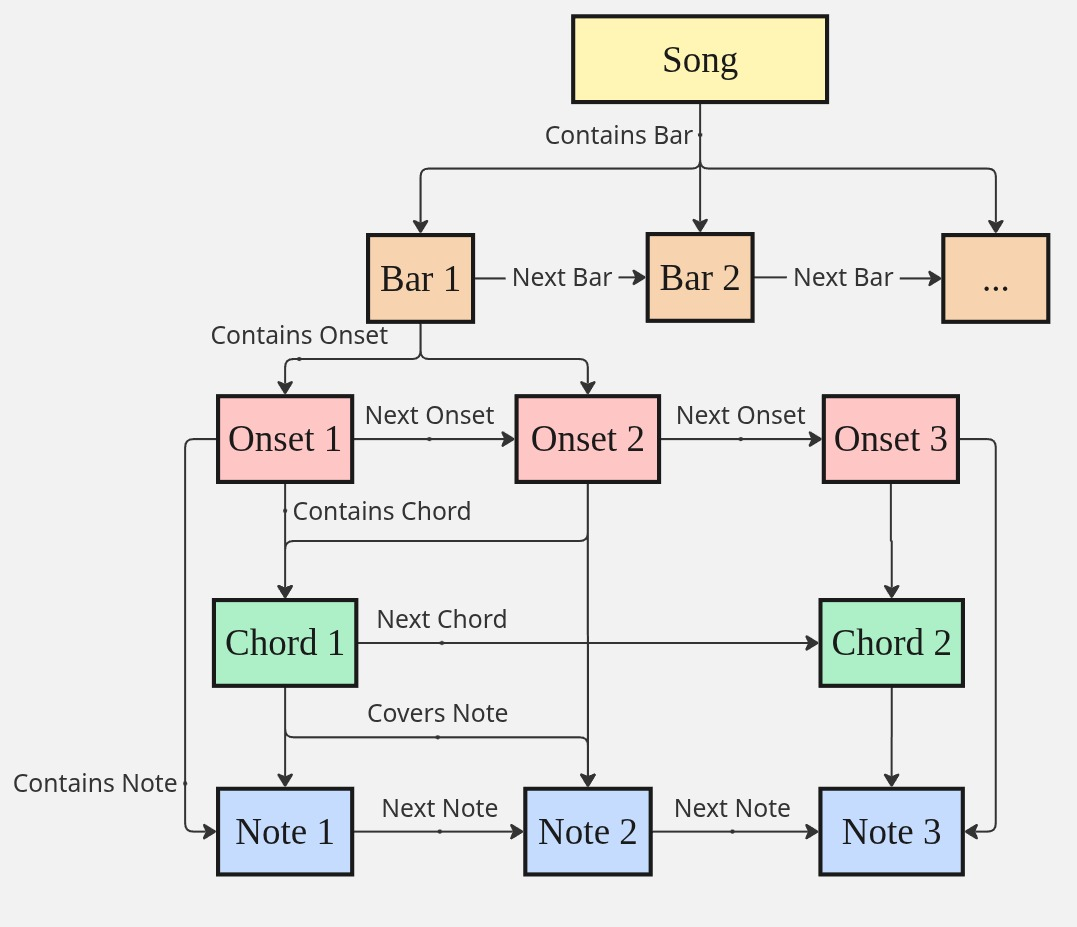
\includegraphics[width=0.96\columnwidth,height=0.63\textheight,keepaspectratio]{graph_hierarchy_edges.jpg}\\[0.12cm]
			{\fontsize{10}{12}\selectfont \textbf{Схема иерархии и типов связей}}
		\end{center}
		\column{0.5\textwidth}
		\begin{center}
			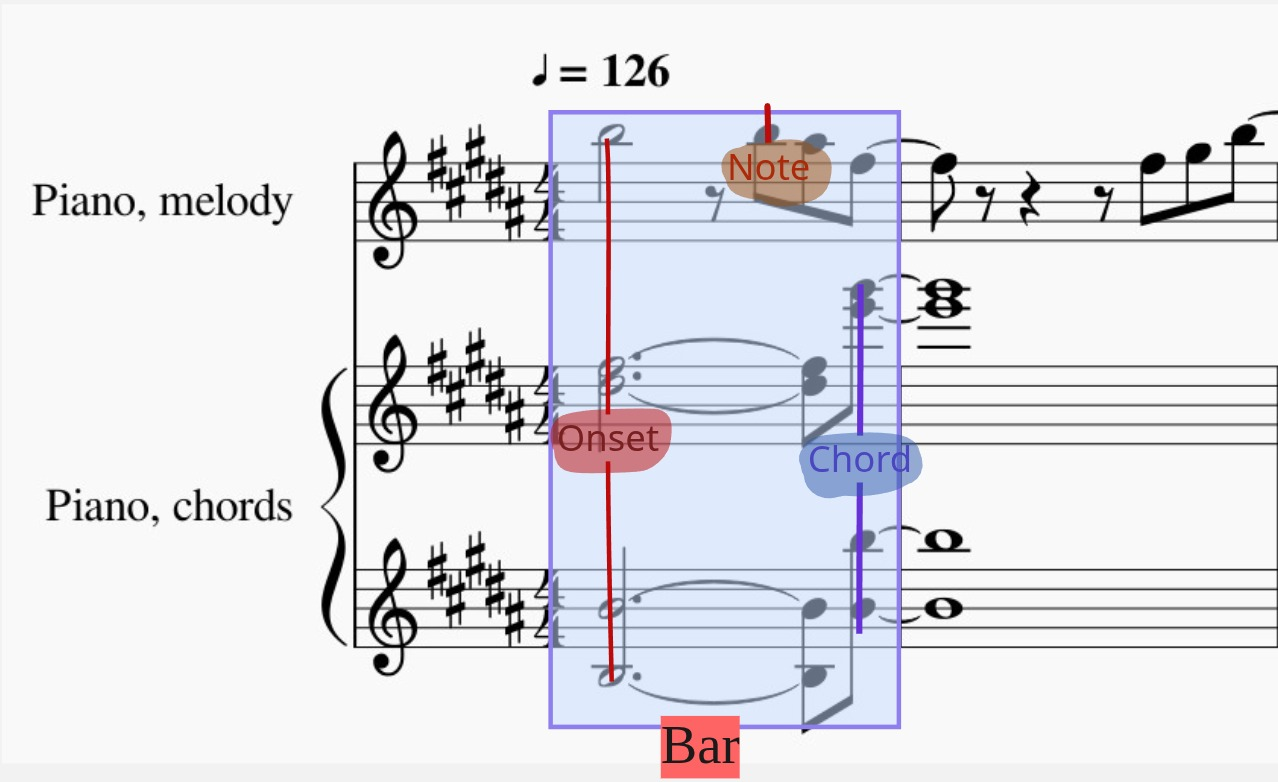
\includegraphics[width=0.96\columnwidth,height=0.63\textheight,keepaspectratio]{graph_hierarchy_score.jpg}\\[0.12cm]
			{\fontsize{10}{12}\selectfont \textbf{Иерархия в формате нотной записи}}
		\end{center}
	\end{columns}
\end{frame}

\begin{frame}
\frametitle{GNN Critic}
\framesubtitle{Пример искажений треков}
\begin{center}
	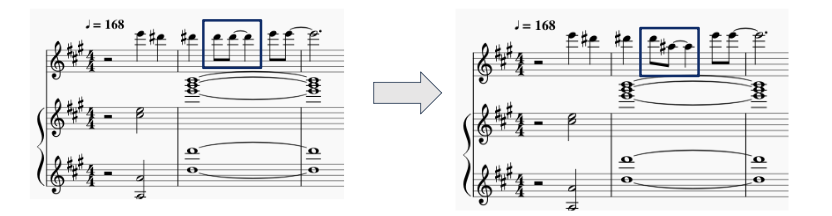
\includegraphics[width=0.95\textwidth,height=0.38\textheight,keepaspectratio]{Screenshot From 2026-05-19 15-45-20.png}\\[0.12cm]
	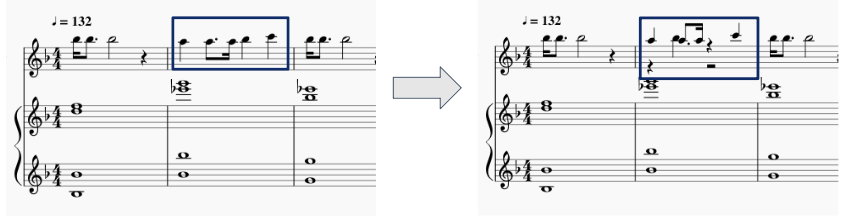
\includegraphics[width=0.95\textwidth,height=0.38\textheight,keepaspectratio]{Screenshot From 2026-05-19 15-45-47.png}\\[0.03cm]
	{\fontsize{10}{12}\selectfont \textbf{Нотная запись до и после искажений}}
\end{center}
\end{frame}

\begin{frame}
\frametitle{GNN Critic}
\framesubtitle{Схема применения графового критика}
\centering
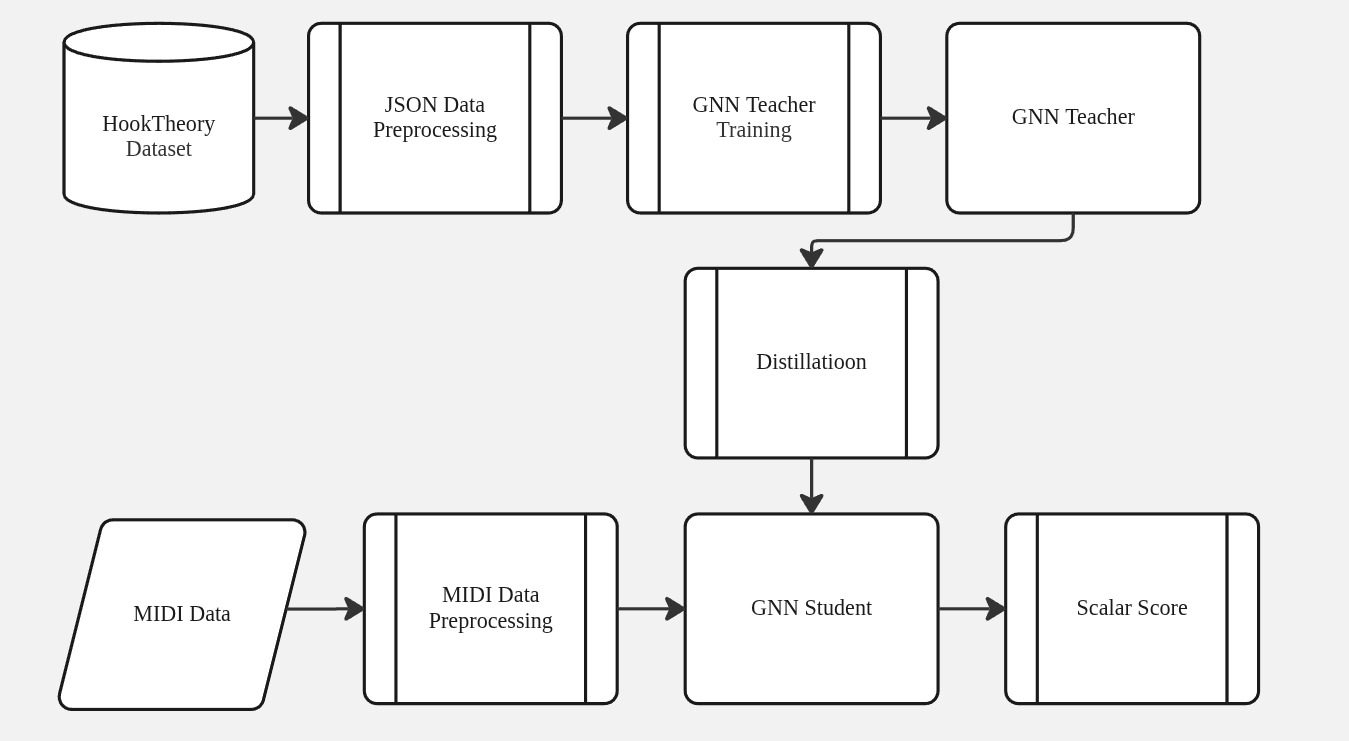
\includegraphics[width=0.9\textwidth,height=0.68\textheight,keepaspectratio]{GNNCriticScheme.jpg}\par
\vspace{0.08cm}
{\fontsize{10}{12}\selectfont \textbf{Схема применения графового критика}}
\end{frame}

\begin{frame}
\frametitle{GNN Critic}
\framesubtitle{Схема обучения графового учителя}
\begin{columns}[c,totalwidth=\textwidth]
	\column{0.24\textwidth}
	{\fontsize{10}{9.6}\selectfont\raggedright
	$\mathcal{G}$ -- исходный граф
	\\[0.15cm]
	$\widetilde{\mathcal{G}}$ -- искаженный граф
	\\[0.15cm]
	Модель обучается выполнять условие:
	\[
	\begin{gathered}
	s_\theta(\mathcal{G}) > s_\theta(\widetilde{\mathcal{G}})
	\end{gathered}
	\]
	}
	\column{0.76\textwidth}
	\centering
	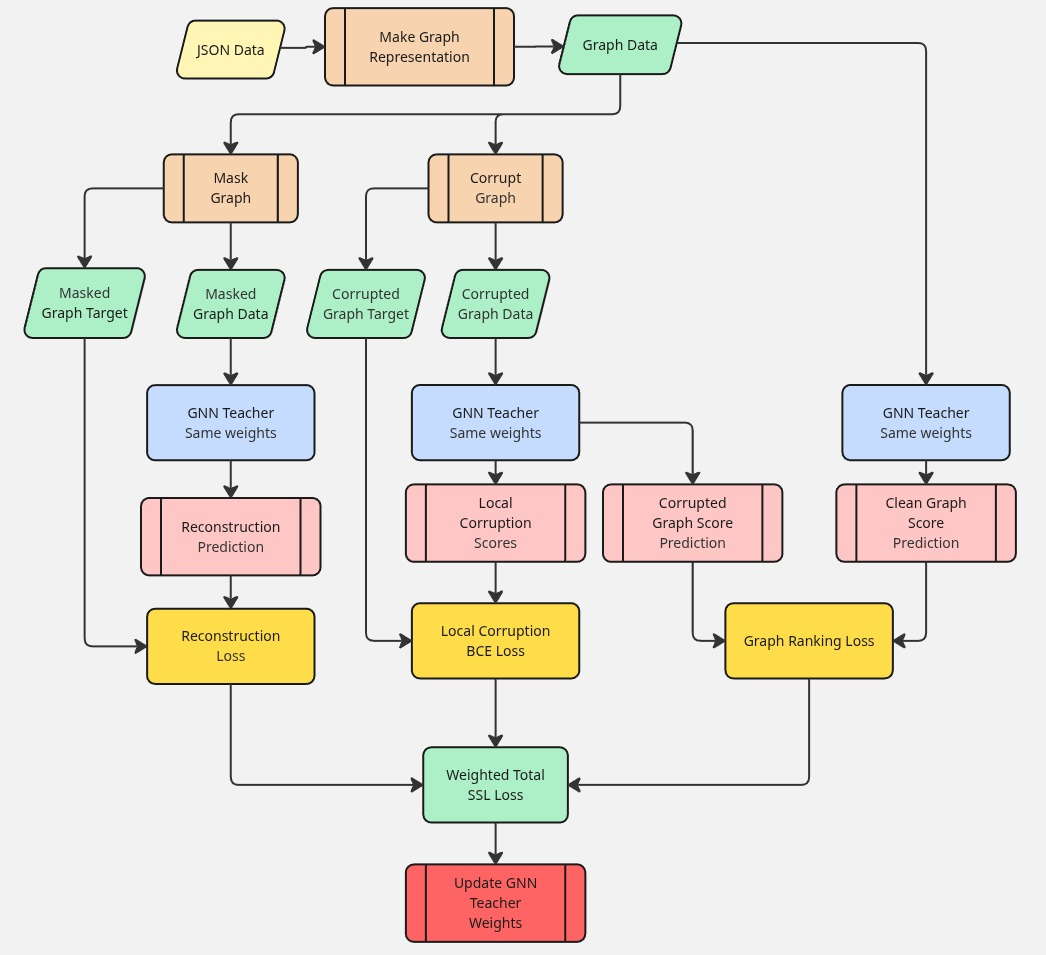
\includegraphics[width=0.8\columnwidth,height=0.72\textheight]{teacher_training_scheme.jpg}\\[0.08cm]
	{\fontsize{10}{12}\selectfont \textbf{Схема обучения графового учителя}}
\end{columns}
\end{frame}

\begin{frame}
\frametitle{GNN Critic}
\framesubtitle{Схема обучения графового ученика}
\centering
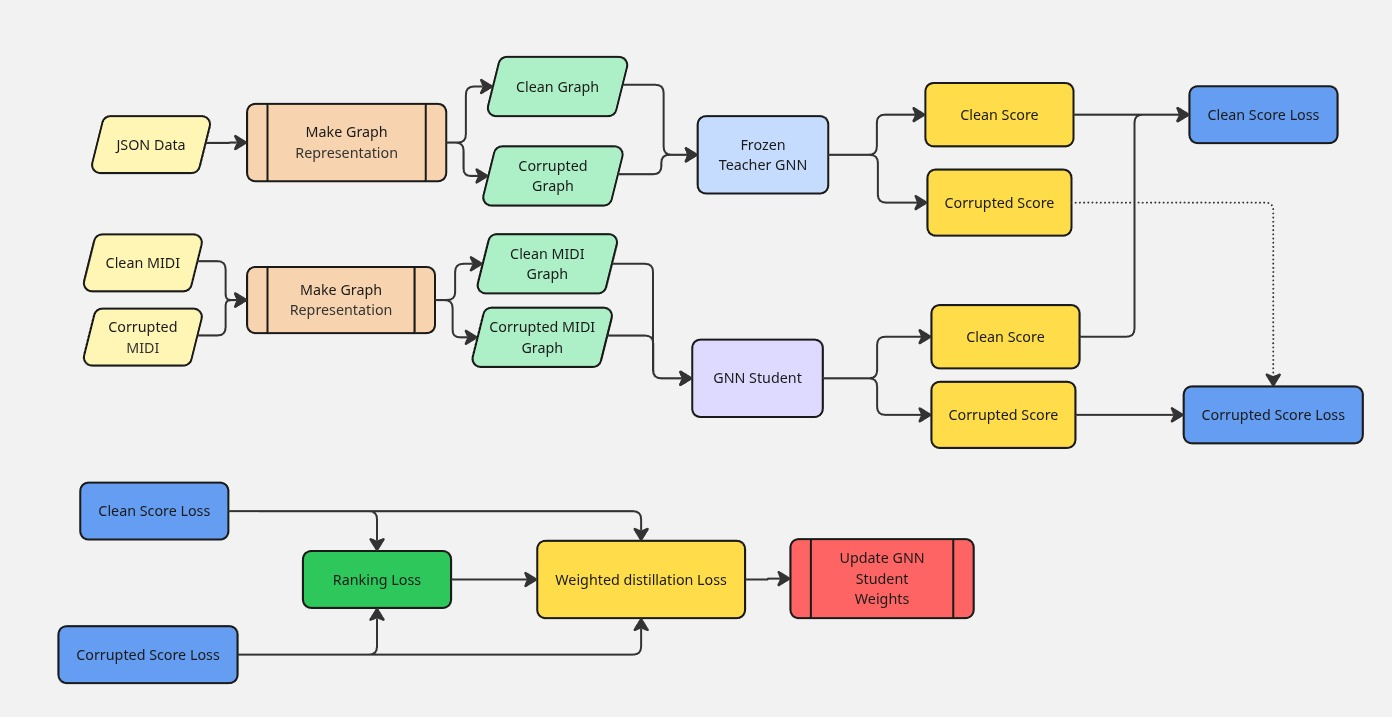
\includegraphics[width=0.9\textwidth,height=0.68\textheight,keepaspectratio]{student_training_scheme.jpg}\par
\vspace{0.08cm}
{\fontsize{10}{12}\selectfont \textbf{Общая схема обучения графового ученика}}
\end{frame}

\begin{frame}
\frametitle{GNN Critic}
\framesubtitle{Механизм определения аккордов из MIDI}
\vspace{0.05cm}
\definecolor{MidiHeader}{RGB}{222,222,222}
\definecolor{MidiRowA}{RGB}{198,207,230}
\definecolor{MidiRowB}{RGB}{228,232,242}
\begin{columns}[T,totalwidth=\textwidth]
	\column{0.27\textwidth}
	{\fontsize{18}{22}\selectfont\raggedright
	Ноты на входе:\\[0.1cm]
	\textbf{C - E - G - B}
	}
	\column{0.73\textwidth}
	\centering
	{\fontsize{9.5}{11.5}\selectfont
	\setlength{\tabcolsep}{4pt}
	\renewcommand{\arraystretch}{1.45}
	\resizebox{\columnwidth}{!}{%
	\begin{tabular}{>{\centering\arraybackslash}p{3.6cm}
		>{\centering\arraybackslash}p{3.6cm}
		>{\centering\arraybackslash}p{3.6cm}}
	\rowcolor{MidiHeader}
	Возможная интерпретация & Функция & Лад / тональный контекст \\
	\rowcolor{MidiRowA}
	Cmaj7 & I --- тоника & C Ionian \\
	\rowcolor{MidiRowB}
	Em($\flat$13) & i --- модальная тоника & E Phrygian \\
	\rowcolor{MidiRowA}
	G6sus4 (или G(add4,6)) & I с суспензией / тоническое зависание & G Ionian \\
	\rowcolor{MidiRowB}
	Cmaj7 & III --- медиантовая окраска & A melodic minor \\
	\rowcolor{MidiRowA}
	B$\varnothing$(add$\flat$9) (условная неполная трактовка) & i$\varnothing$ --- локрийская тоника & B Locrian \\
	\rowcolor{MidiRowB}
	Cmaj7 & V --- доминантовая ступень без классического доминантового напряжения & F Lydian \\
	\end{tabular}
	}
	}
\end{columns}
\end{frame}

\begin{frame}
\frametitle{GNN Critic}
\framesubtitle{Аккордовый оценщик}
\vspace{0.2cm}
{\fontsize{15}{19}\selectfont
Аккордовый оценщик выбирает кандидата с наибольшим количеством очков соответствия, которые считаются как:
}
\[
q(c, P_w)
=
q_{+}(c, P_w)
-
q_{-}(c, P_w),
\]
\vspace{0.1cm}
{\fontsize{13}{17}\selectfont
\begin{itemize}
	\setlength{\itemsep}{0.18cm}
	\item $P_w$ --- наблюдаемые ноты;
	\item $c$ --- аккордовый кандидат;
	\item $q_{+}$ --- \hyperlink{positive-score}{положительный вклад} объяснённых признаков;
	\item $q_{-}$ --- \hyperlink{negative-score}{штрафы за несоответствия}.
\end{itemize}
}
\end{frame}



\begin{frame}
\frametitle{GNN Critic}
\framesubtitle{Сравнение механизмов искажения}
\begin{table}
\centering
\footnotesize
{\large\textbf{Сравнение случайных и теоретически обоснованных искажений}}\\[0.2cm]
\label{tab:1}
\resizebox{\textwidth}{!}{%
\begin{tabular}{@{}lllll@{}}
\toprule
\textit{Corruption family} & \textit{Pooling} & \textit{Best rank acc} $\uparrow$ \\
\midrule
\textit{Theory-aware} & \textit{mean\_max} & \textbf{1.0000} \\
\textit{Graph} & \textit{mean\_max}  & 0.8750 \\
\bottomrule
\end{tabular}%
}
\end{table}
\end{frame}

\begin{frame}
\frametitle{GNN Critic}
\framesubtitle{Обзор обобщающей способности критика}
\begin{table}[htbp]
{\Large\textbf{Проверка обобщения teacher-модели на OOD-corruptions}}\\[0.25cm]
\label{tab:ood-corruption-groups}
\centering
\small
\setlength{\tabcolsep}{4pt}
\renewcommand{\arraystretch}{1.25}
\begin{tabular}{@{}p{3.5cm}p{1.7cm}p{1cm}p{6.2cm}@{}}
\toprule
\textit{Group} & \textit{Mean gap} & \textit{Global RankAcc} & \textit{Interpretation} \\
\midrule
\textit{Harmful OOD corruptions} & 0.6649 & 0.5504 & Новые вредные искажения в среднем понижают \textit{score} \\
\textit{Benign transformations} & 0.0110 & 0.5012 & Безвредные преобразования почти не создают систематический штраф \\
\bottomrule
\end{tabular}
\end{table}
\end{frame}

\begin{frame}
\frametitle{GNN Critic}
\framesubtitle{Staged training}
\begin{table}[htbp]
\caption{\textit{Staged training}}
\label{tab:3}
\centering
\scriptsize
\resizebox{\textwidth}{!}{%
\begin{tabular}{@{}llllllllll@{}}
\toprule
\textit{Training mode} & \textit{Best IntraAcc} $\uparrow$ & \textit{Best InterAcc} $\uparrow$ & \textit{BinaryAcc} $\uparrow$ \\
\midrule
\textit{MLM} $\to$ \textit{corruption}   & \textbf{0.9118} & \textbf{0.8994} & 0.7486 \\
\textit{Corruption from scratch} & 0.9007 & 0.8962 & \textbf{0.7489} \\
\bottomrule
\end{tabular}%
}
\end{table}
\MetricLegend
\end{frame}

\begin{frame}
\frametitle{GNN Critic}
\framesubtitle{Feature ablation}
\begin{table}[htbp]
\caption{\textit{Feature ablation}: \textit{dynamic weighting}, \textit{HGT} и \textit{learned logit fusion}}
\label{tab:4}
\centering
\scriptsize
\resizebox{\textwidth}{!}{%
\begin{tabular}{@{}llllllllll@{}}
\toprule
\textit{Variant} & \textit{Backbone} & \textit{Dynamic weights} & \textit{Logit fusion} & \textit{Best IntraAcc} $\uparrow$ & \textit{Best InterAcc} $\uparrow$ & \textit{BinaryAcc} $\uparrow$ \\
\midrule
\textit{Baseline} & \textit{SAGE} & \textit{no} & \textit{no} & 0.8547 & 0.8472 & 0.7668 \\
\textit{HGT} & \textit{HGT} & \textit{no} & \textit{no}  & 0.8410 & 0.8409 & 0.7537 \\
\textit{Dynamic weights} & \textit{SAGE} & \textit{yes} & \textit{no}  & 0.8530 & \textbf{0.8494} & \textbf{0.7731} \\
\textit{Learned logit fusion} & \textit{SAGE} & \textit{no} & \textit{yes} & 0.8408 & \textbf{0.8523} & \textbf{0.7761} \\
\bottomrule
\end{tabular}%
}
\end{table}
\MetricLegend
\end{frame}

\begin{frame}
\frametitle{GNN Critic}
\framesubtitle{Финальная teacher-конфигурация}
\begin{table}[htbp]
\caption{Финальная \textit{teacher}-конфигурация}
\label{tab:5}
\centering
\scriptsize
\resizebox{\textwidth}{!}{%
\begin{tabular}{@{}llllllllllll@{}}
\toprule
\textit{Backbone} & \textit{Dynamic weights} & \textit{Logit fusion} & \textit{Hidden / layers} & \textit{Pooling} & \textit{Local context} & \textit{MLM / corr epochs} & \textit{Best IntraAcc} $\uparrow$ & \textit{Best InterAcc} $\uparrow$ & \textit{BinaryAcc} $\uparrow$ \\
\midrule
\textit{SAGE} & \textit{yes} & \textit{yes} & 256 / 4 & \textit{mean\_max} & \textit{attention} & 30 / 39 & \textbf{0.9275} & \textbf{0.9250} & \textbf{0.8456} \\
\bottomrule
\end{tabular}%
}
\end{table}
\MetricLegend
\end{frame}

\begin{frame}
\frametitle{GNN Critic}
\framesubtitle{Scoring для восстановления аккордов из MIDI}
\begin{table}[htbp]
\caption{Сравнение ручного и обучаемого \textit{scoring} для восстановления аккордов из \textit{MIDI}}
\label{tab:chord-prediction-scoring}
\centering
\scriptsize
\resizebox{\textwidth}{!}{%
\begin{tabular}{@{}lrrrrrrr@{}}
\toprule
\textit{Scoring} & \textit{Top-1 exact} $\uparrow$ & \textit{Top-5 contains GT} $\uparrow$ & \textit{Root acc} $\uparrow$ & \textit{Type acc} $\uparrow$ & \textit{Root+Type acc} $\uparrow$ & \textit{Mode acc} $\uparrow$ & \textit{Inversion acc} $\uparrow$ \\
\midrule
\textit{Learned weights} & \textbf{0.9216} & \textbf{0.9907} & \textbf{0.9753} & \textbf{0.9864} & \textbf{0.9690} & \textbf{0.9324} & \textbf{0.9811} \\
\textit{Manual} & 0.7641 & 0.9184 & 0.9249 & 0.8368 & 0.8147 & 0.9061 & 0.9213 \\
\bottomrule
\end{tabular}%
}
\end{table}
\end{frame}

\begin{frame}
\frametitle{GNN Critic}
\framesubtitle{Качество восстановления аккордов по типам}
\begin{table}[htbp]
\caption{Качество восстановления аккордов по типам}
\label{tab:chord-type-accuracy}
\centering
\footnotesize
\begin{tabular}{@{}lrr@{}}
\toprule
\textit{Type} & \textit{Manual weights} $\uparrow$ & \textit{Learned weights} $\uparrow$ \\
\midrule
\textit{triad / 5} & 0.915 & \textbf{0.938} \\
\textit{seventh / 7} & 0.227 & \textbf{0.867} \\
\textit{ninth / 9} & 0.000 & \textbf{0.850} \\
\textit{eleventh / 11} & 0.000 & \textbf{0.886} \\
\textit{thirteenth / 13} & 0.000 & \textbf{0.089} \\
\bottomrule
\end{tabular}
\end{table}
\end{frame}

\begin{frame}
\frametitle{GNN Critic}
\framesubtitle{Промежуточная дистилляция}
\vspace{-0.28cm}
{\fontsize{9.6}{11}\selectfont
\[
\begin{aligned}
\mathcal{L}
={}&
\lambda_s \mathcal{L}_{score}
+
\lambda_r \mathcal{L}_{rank}
+
\lambda_m \mathcal{L}_{margin}
+
\lambda_g \mathcal{L}_{graph}
+
\lambda_t \mathcal{L}_{type}
+
\lambda_l \mathcal{L}_{local}.
\end{aligned}
\]
\vspace{-0.35cm}
\begin{columns}[T,totalwidth=\textwidth]
	\column{0.48\textwidth}
	\[
	\mathcal{L}_{graph}
	=
	\left\|
	P_g z_G^{S} - z_G^{T}
	\right\|_2^2
	\]
	\vspace{-0.28cm}
	\[
	\mathcal{L}_{type}
	=
	\sum_{\tau}
	\left\|
	P_\tau z_{\tau}^{S} - z_{\tau}^{T}
	\right\|_2^2
	\]
	\vspace{-0.28cm}
	\[
	\mathcal{L}_{local}
	=
	\left\|
	P_l u^{S} - u^{T}
	\right\|_2^2
	\]
	\column{0.5\textwidth}
	\raggedright
	$z_G^{S}$ и $z_G^{T}$ --- графовые \textit{embeddings} \textit{student}- и \textit{teacher}-моделей.\\[0.08cm]
	$z_{\tau}^{S}$ и $z_{\tau}^{T}$ --- \textit{pooled}-представления по типам вершин.\\[0.08cm]
	$u^{S}$ и $u^{T}$ --- локальные \textit{summary}-признаки.\\[0.08cm]
	Матрицы $P_g$, $P_\tau$, $P_l$ являются \textit{projection adapters}, позволяющими сопоставить пространства \textit{student} и \textit{teacher}.
\end{columns}
}
\end{frame}

\begin{frame}
\frametitle{GNN Critic}
\framesubtitle{Дистилляция промежуточных представлений}
\begin{table}[htbp]
\caption{Влияние дистилляции промежуточных представлений \textit{teacher}-модели}
\label{tab:student-intermediate-ablation}
\centering
\scriptsize
\resizebox{\textwidth}{!}{%
\begin{tabular}{@{}lrrrrrr@{}}
\toprule
\textit{Variant} & \textit{Batch rank acc} $\uparrow$ & \textit{Spearman} $\uparrow$ & \textit{Pearson} $\uparrow$ & \textit{MAE} $\downarrow$ & \textit{Score distill loss} $\downarrow$ \\
\midrule
\textit{Intermediate} & \textbf{0.6787} & \textbf{0.4173} & \textbf{0.3588} & \textbf{2.3121} & \textbf{3.7560} \\
\textit{No intermediate} & 0.6111 & 0.2712 & 0.1728 & 2.5432 & 4.2046 \\
\bottomrule
\end{tabular}%
}
\end{table}
{\fontsize{6.9}{7.8}\selectfont
\textit{Batch rank acc} --- доля корректных сравнений между всеми положительными и отрицательными примерами внутри батча.\\[0.03cm]
\textit{Spearman} --- ранговая корреляция между оценками \textit{student} и \textit{teacher}.\\[0.03cm]
\textit{Pearson} --- линейная корреляция между этими оценками.\\[0.03cm]
}
\end{frame}

\begin{frame}
\frametitle{GNN Critic}
\framesubtitle{Финальное сравнение observer-конфигураций}
\begin{table}[htbp]
\caption{Финальное сравнение \textit{observer}-конфигураций}
\label{tab:observer-final-comparison}
\centering
\scriptsize
\resizebox{\textwidth}{!}{%
\begin{tabular}{@{}lllrrrrrr@{}}
\toprule
\textit{Observer variant} & \textit{Intermediate losses}  & \textit{Pair rank acc} $\uparrow$ & \textit{Batch rank acc} $\uparrow$ & \textit{Spearman} $\uparrow$ & \textit{Pearson} $\uparrow$ & \textit{MAE} $\downarrow$ \\
\midrule
\textit{Intermediate} &  \textit{yes}  & \textbf{0.8692} & \textbf{0.8464} & 0.6926 & \textbf{0.6873} & 2.0698 \\
\textit{No intermediate} &  \textit{no}  & 0.8509 & 0.8387 & \textbf{0.7135} & 0.6832 & \textbf{1.4717} \\
\bottomrule
\end{tabular}%
}
\end{table}
\end{frame}

\begin{frame}
\frametitle{Appendix}
\framesubtitle{Распределения тональностей и ладов}
\vspace{0.05cm}
\begin{columns}[c,totalwidth=\textwidth]
	\column{0.5\textwidth}
	\begin{center}
		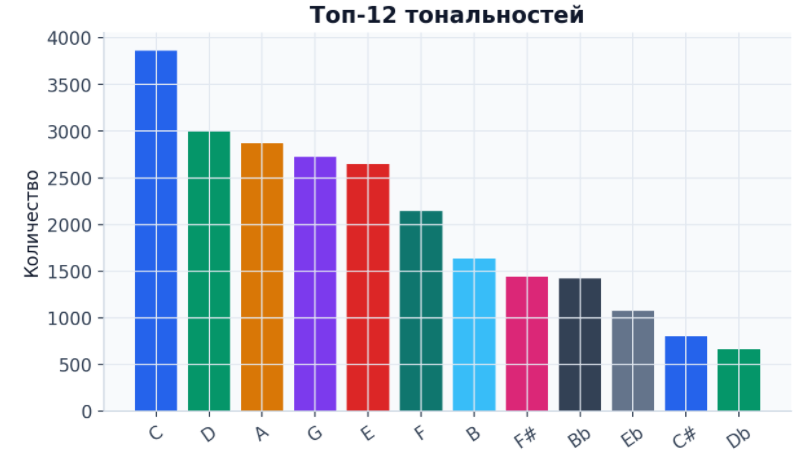
\includegraphics[width=0.96\columnwidth,height=0.62\textheight,keepaspectratio]{key_distribution.png}\\[0.12cm]
		{\fontsize{10}{12}\selectfont \textbf{Распределение тональностей}}
	\end{center}
	\column{0.5\textwidth}
	\begin{center}
		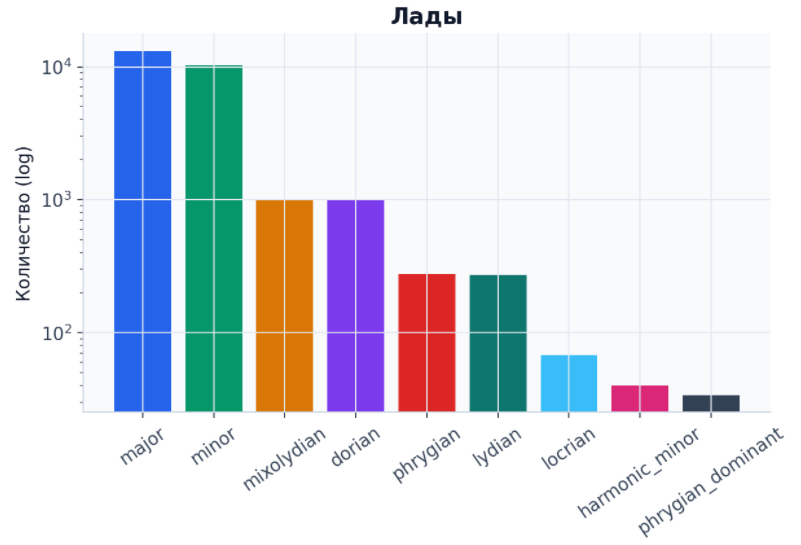
\includegraphics[width=0.96\columnwidth,height=0.62\textheight,keepaspectratio]{mode_distribution.png}\\[0.12cm]
		{\fontsize{10}{12}\selectfont \textbf{Распределение ладов}}
	\end{center}
\end{columns}
\end{frame}

\begin{frame}
\frametitle{Appendix}
\framesubtitle{Распределения ступеней и типов аккордов}
\vspace{0.05cm}
\begin{columns}[c,totalwidth=\textwidth]
	\column{0.5\textwidth}
	\begin{center}
		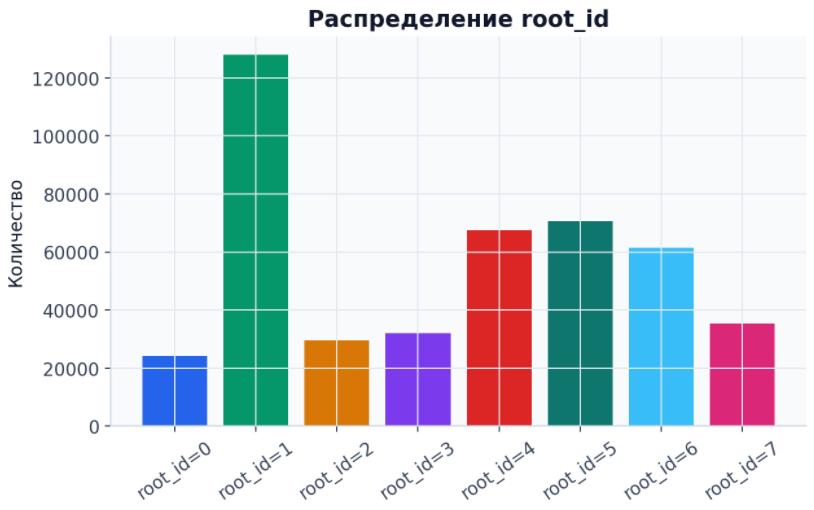
\includegraphics[width=0.96\columnwidth,height=0.62\textheight,keepaspectratio]{chord_degree_distribution.png}\\[0.12cm]
		{\fontsize{10}{12}\selectfont \textbf{Распределение ступеней аккордов}}
	\end{center}
	\column{0.5\textwidth}
	\begin{center}
		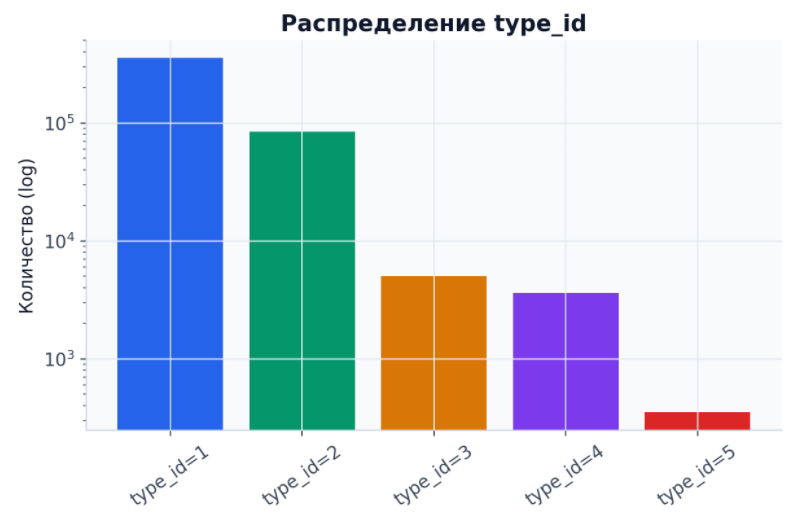
\includegraphics[width=0.96\columnwidth,height=0.62\textheight,keepaspectratio]{chord_type_distribution.png}\\[0.12cm]
		{\fontsize{10}{12}\selectfont \textbf{Распределение типов аккордов}}
	\end{center}
\end{columns}
\end{frame}

\begin{frame}
\frametitle{Appendix}
\framesubtitle{Обучение графового учителя}
\vspace{-0.25cm}
{\fontsize{5.7}{6.5}\selectfont
\setlength{\abovedisplayskip}{1pt}
\setlength{\belowdisplayskip}{1pt}
\begin{columns}[T,totalwidth=\textwidth]
	\column{0.49\textwidth}
	Признаки каждой вершины проецируются в общее скрытое пространство:
	\[
	h_v^{(0)}=\phi_{\tau_v}(x_v),
	\]
	где $\phi_{\tau_v}$ --- \textit{encoder} для типа вершины $\tau_v$, реализованный как \textit{MLP}.

	Для каждого типа ребра $r$ сообщения вычисляются отдельно:
	\[
	m_{u\to v}^{(l,r)}=W_r^{(l)}h_u^{(l)}.
	\]
	Сообщения от соседей агрегируются:
	\[
	m_v^{(l)}=\sum_{r\in R}\operatorname{AGG}_{u\in N_r(v)} m_{u\to v}^{(l,r)}.
	\]
	Состояние вершины обновляется с \textit{residual}-связью, нормализацией и нелинейностью:
	\[
	h_v^{(l+1)}=\operatorname{ReLU}\!\left(\operatorname{LN}\!\left(h_v^{(l)}+m_v^{(l)}\right)\right).
	\]

	После нескольких \textit{GNN}-слоёв модель получает контекстуализированные представления узлов. Затем выполняется \textit{pooling} по типам вершин:
	\[
	g_t=\frac{1}{|V_t|}\sum_{v\in V_t}h_v^{(L)},
	\]
	где $V_t$ --- множество вершин типа $t$.

	\column{0.49\textwidth}
	После объединения векторов разных типов получается общий \textit{embedding} графа:
	\[
	g=\psi\!\left(g_1\Vert g_2\Vert\ldots\Vert g_T\right),
	\]
	где $\Vert$ --- конкатенация, а $\psi$ --- линейная проекция или \textit{MLP}. Итоговая оценка графа:
	\[
	s_\theta(\mathcal{G})=f_{\mathrm{score}}(g).
	\]

	Для обучения используется \textit{contrastive ranking loss}:
	\[
	\mathcal{L}_{\mathrm{rank}}=
	\operatorname{softplus}\!\left(-\left(s_\theta(\mathcal{G})-s_\theta(\widetilde{\mathcal{G}})-m\right)\right),
	\]
	где $m$ --- \textit{margin}. Функция штрафует модель, если \textit{score} искажённого графа слишком близок к \textit{score} исходного или превосходит его.

	Дополнительно может использоваться бинарная классификационная компонента:
	\[
	\mathcal{L}_{\mathrm{bin}}=\frac{1}{2}\left(
	\operatorname{BCE}\!\left(s_\theta(\mathcal{G}),1\right)+
	\operatorname{BCE}\!\left(s_\theta(\widetilde{\mathcal{G}}),0\right)
	\right).
	\]
	Общая функция потерь учителя:
	\[
	\mathcal{L}_{\mathrm{teacher}}=
	\lambda_{\mathrm{rank}}\mathcal{L}_{\mathrm{rank}}+
	\lambda_{\mathrm{bin}}\mathcal{L}_{\mathrm{bin}}+
	\lambda_{\mathrm{local}}\mathcal{L}_{\mathrm{local}}+
	\lambda_{\mathrm{rec}}\mathcal{L}_{\mathrm{rec}}.
	\]
\end{columns}
}
\end{frame}

\begin{frame}
\frametitle{Appendix}
\framesubtitle{Обучение графового ученика}
\vspace{-0.25cm}
{\fontsize{6.1}{7}\selectfont
\setlength{\abovedisplayskip}{1pt}
\setlength{\belowdisplayskip}{1pt}
\begin{columns}[T,totalwidth=\textwidth]
	\column{0.49\textwidth}
	После построения \textit{MIDI}-графа ученик использует компактную гетерогенную \textit{GNN}. Для каждой вершины строится начальное представление:
	\[
	z_v^{(0)}=\phi_{\tau_v}(x_v),
	\]
	после чего несколько графовых слоёв обновляют его через сообщения от соседей:
	\[
	z_v^{(l+1)}=\sigma\!\left(\operatorname{LN}\!\left(
	z_v^{(l)}+\sum_r\operatorname{AGG}_{u\in N_r(v)}W_r^{(l)}z_u^{(l)}
	\right)\right).
	\]
	Далее применяется \textit{pooling} по вершинам и строится \textit{embedding} \textit{MIDI}-графа:
	\[
	z_G=\operatorname{Pool}\!\left(\{z_v^{(L)}\}_{v\in V_M}\right).
	\]
	Итоговая оценка ученика равна:
	\[
	s_\varphi(\mathcal{G}_M)=f_{\mathrm{student}}(z_G).
	\]

	\column{0.49\textwidth}
	Ученик обучается не на ручных метках, а на оценках учителя. Если учитель присваивает музыкальному фрагменту \textit{score} $s_\theta(\mathcal{G})$, то ученик минимизирует ошибку дистилляции:
	\[
	\mathcal{L}_{\mathrm{distill}}=
	\left|s_\varphi(\mathcal{G}_M)-s_\theta(\mathcal{G})\right|,
	\]
	или её сглаженный вариант:
	\[
	\mathcal{L}_{\mathrm{distill}}=
	\operatorname{SmoothL1}\!\left(s_\varphi(\mathcal{G}_M),s_\theta(\mathcal{G})\right).
	\]
	Для пар \textit{clean/corrupted} дополнительно используется \textit{ranking loss}:
	\[
	\mathcal{L}_{\mathrm{student\text{-}rank}}=
	\operatorname{softplus}\!\left(-\left(s_\varphi(\mathcal{G}_M)-s_\varphi(\widetilde{\mathcal{G}}_M)\right)\right).
	\]
\end{columns}
}
\end{frame}

\begin{frame}
\frametitle{Appendix}
\framesubtitle{Положительная часть аккордового score}
\hypertarget{positive-score}{}
\vspace{-0.15cm}
{\fontsize{9.5}{11.5}\selectfont
\textbf{Компоненты положительной части аккордового \textit{score}}\\[0.08cm]
\setlength{\tabcolsep}{4pt}
\renewcommand{\arraystretch}{1.18}
\begin{tabular}{@{}p{0.34\textwidth}p{0.58\textwidth}@{}}
\toprule
\textit{Компонента} & \textit{Интерпретация} \\
\midrule
$\operatorname{mode\_match}(c)$ & Совпадение лада \\
$\operatorname{bass\_match}(c)$ & Совпадение басовой ноты \\
$|P_w \cap B(c)|$ & Количество совпадающих нот \\
$\operatorname{explained\_extras}(c, P_w)$ & Надстройки \\
\bottomrule
\end{tabular}
}
\end{frame}

\begin{frame}
\frametitle{Appendix}
\framesubtitle{Штрафная часть аккордового score}
\hypertarget{negative-score}{}
\vspace{-0.1cm}
{\fontsize{9.5}{11.5}\selectfont
\textbf{Компоненты штрафной части аккордового \textit{score}}\\[0.08cm]
\setlength{\tabcolsep}{4pt}
\renewcommand{\arraystretch}{1.22}
\begin{tabular}{@{}p{0.38\textwidth}p{0.56\textwidth}@{}}
\toprule
\textit{Компонента} & \textit{Интерпретация} \\
\midrule
$\operatorname{Unexplained}(c, P_w)$ & Ноты которые не объясняются кандидатом \\
$\operatorname{MissingCore}(c, P_w)$ & Ноты кандидата которых нет в MIDI \\
$\operatorname{borrowed\_mode\_penalty}(c)$ & Штраф за заимствованный лад \\
$\operatorname{mode\_distance}(c)$ & Штраф за расстояние до заимствованного лада \\
$\operatorname{body\_size\_penalty}(c)$ & Штраф за размер аккорда \\
$\operatorname{complexity\_penalty}(c)$ & Штрафы за добавленные ступени, задержания, альтерации и пропущенные обязательные тона. \\
\bottomrule
\end{tabular}
}
\end{frame}

\begin{frame}
\frametitle{Appendix}
\framesubtitle{Пример применения аккордового оценщика}
\vspace{-0.25cm}
{\fontsize{8.5}{10}\selectfont
Пусть в момент времени $t$ наблюдаются \textit{MIDI}-ноты
$C - E - G - B\flat$, тогда $P_t=\{C,E,G,B\flat\}$.
\vspace{0.08cm}
\setlength{\tabcolsep}{2.5pt}
\renewcommand{\arraystretch}{1.16}
\resizebox{\textwidth}{!}{%
\begin{tabular}{@{}p{0.17\textwidth}p{0.29\textwidth}p{0.31\textwidth}p{0.19\textwidth}@{}}
\toprule
\textit{Кандидат} & \textit{Тело аккорда} & \textit{Совпадения и штрафы} & \textit{Итог} \\
\midrule
\textbf{$C7$} &
$B(C7)=\{C,E,G,B\flat\}$ &
$P_t\cap B(C7)=\{C,E,G,B\flat\}$;\newline
$\operatorname{MissingCore}=\varnothing$;\newline
$\operatorname{Unexplained}=\varnothing$ &
Высокий \textit{score}: полный доминантсептаккорд. \\
\midrule
\textbf{$C$ major} &
$B(C)=\{C,E,G\}$ &
Трезвучие объясняется, но $B\flat$ остаётся необъяснённым:\newline
$\operatorname{Unexplained}=\{B\flat\}$ &
\textit{Score} ниже, если $B\flat$ не считается допустимой добавленной или альтерированной ступенью. \\
\midrule
\textbf{$Am7\flat5/C$} &
$B(Am7\flat5)=\{A,C,E\flat,G\}$ &
Есть $C$ и $G$, но отсутствуют $A$ и $E\flat$; вместо $E\flat$ наблюдается $E$:\newline
$\operatorname{MissingCore}=\{A,E\flat\}$ &
Совпадение баса $C$ не компенсирует штрафы: \textit{score} ниже, чем у $C7$. \\
\bottomrule
\end{tabular}%
}
}
\end{frame}

\end{document}
